\documentclass{beamer}
%
% Choose how your presentation looks.
%
% For more themes, color themes and font themes, see:
% http://deic.uab.es/~iblanes/beamer_gallery/index_by_theme.html
%

% Change font for math mode
%\usepackage{mathpazo}
%\renewcommand\rmdefault{hpv}

\mode<presentation>
{
  \usetheme{Luebeck}      % or try Darmstadt, Madrid, Warsaw, ...
  \usecolortheme{seahorse} % or try albatross, beaver, crane, ...
  \usefonttheme{default}  % or try serif, structurebold, ...
  \setbeamertemplate{navigation symbols}{}
  \setbeamertemplate{caption}[numbered]
} 
\usepackage[default]{comfortaa}
\usepackage[T1]{fontenc} 
\renewcommand{\rmdefault}{cmr}
\renewcommand{\sfdefault}{cmss}
\renewcommand{\ttdefault}{cmtt}
\usepackage[english]{babel}
\usepackage[utf8x]{inputenc}
\usepackage{mathtools}
\DeclarePairedDelimiter\abs{\lvert}{\rvert}%
\DeclarePairedDelimiter\norm{\lVert}{\rVert}%
\usepackage{amsmath}
\DeclareMathOperator*{\argmax}{arg\,max}
\DeclareMathOperator*{\argmin}{arg\,min}
\usepackage{caption}

\title[Linear Classification]{Elements of Statistical Learning 4: \\
Linear Methods for Classification}
\author{Fabian Hainzl}
\institute{appliedAI}
\date{1.8.2019}

\begin{document}

\begin{frame}
  \titlepage
\end{frame}

%\begin{frame}{Outline}
%  \tableofcontents
%\end{frame}

\begin{frame}{Notation}

{\small \textit{Notation in these slides follows Elements of Statistical Learning}}
\vspace{0.5cm}
\begin{tabular}{|c|c|}
\hline
$G(x)$ & Predictor \\
\hline
$p_k(x)$ & $Pr(G=k|X=x)$ \\
\hline
$\pi_k$ & $Pr(G=k)$ \\
\hline
$\hat{f}_k(x) = \hat{\beta}_{k0}+\hat{\beta}_k^Tx$ & Linear model for k-th output dimension \\
\hline
K & Number of classes \\
\hline
N & Number of samples \\
\hline
\end{tabular}
\end{frame}

\begin{frame}{Classification}
Two approaches to supervised learning:
\begin{itemize}
\item Regression: Continuous output variable
\item Classification: Discrete output variable
\end{itemize}
\vspace{0.5cm}
Goal of classification
\begin{itemize}
\item Divide input space into a collection of regions with constant classification
\end{itemize}
\vspace{0.5cm}
Linear Regression
%\pause
\begin{itemize}
\item Linear dependence of output on the weights
\end{itemize}
\vspace{0.5cm}
Linear Classification
%\pause
\begin{itemize}
\item Linear decision boundaries
\end{itemize}

\end{frame}

\begin{frame}{Decision Boundary}

\vspace{0.2cm}
Decision boundaries 
\begin{itemize}
\item Boundaries between regions of different classes
\item Points of input space where several classes have same probability
\end{itemize}
\vspace{0.2cm}
Definition of decision boundary for binary classification:
\begin{equation*}
\{ x:(\hat{\beta}_{k0} - \hat{\beta}_{m0}) + 
(\hat{\beta}_{k} - \hat{\beta}_{m})^Tx = 0\}
\end{equation*}
\end{frame}


\begin{frame}{Linear classification}
Linear classification:
\begin{itemize}
\item[•] Decision boundaries are hyperplanes
\end{itemize}
This is the case if 
\begin{itemize}
\item[•] posterior probability $Pr(G=k|X=x)$ is linear in x
\item[•] monotone transformation of posterior probability is linear
\end{itemize}
\end{frame}


\begin{frame}{Generalization to non-linear decision boundaries}
Augment feature space by adding squares and cross-products of features

\vspace{0.2cm}
Example for 2 dimensions:
\begin{columns}
\begin{column}{0.5\textwidth}
\begin{center}
$X_1,X_2$
\end{center}
\end{column}
\begin{column}{0.5\textwidth}
\begin{center}
$X_1,X_2,X_1^2, X_2^2, X_1 X_2$
\end{center}
\end{column}
\end{columns}

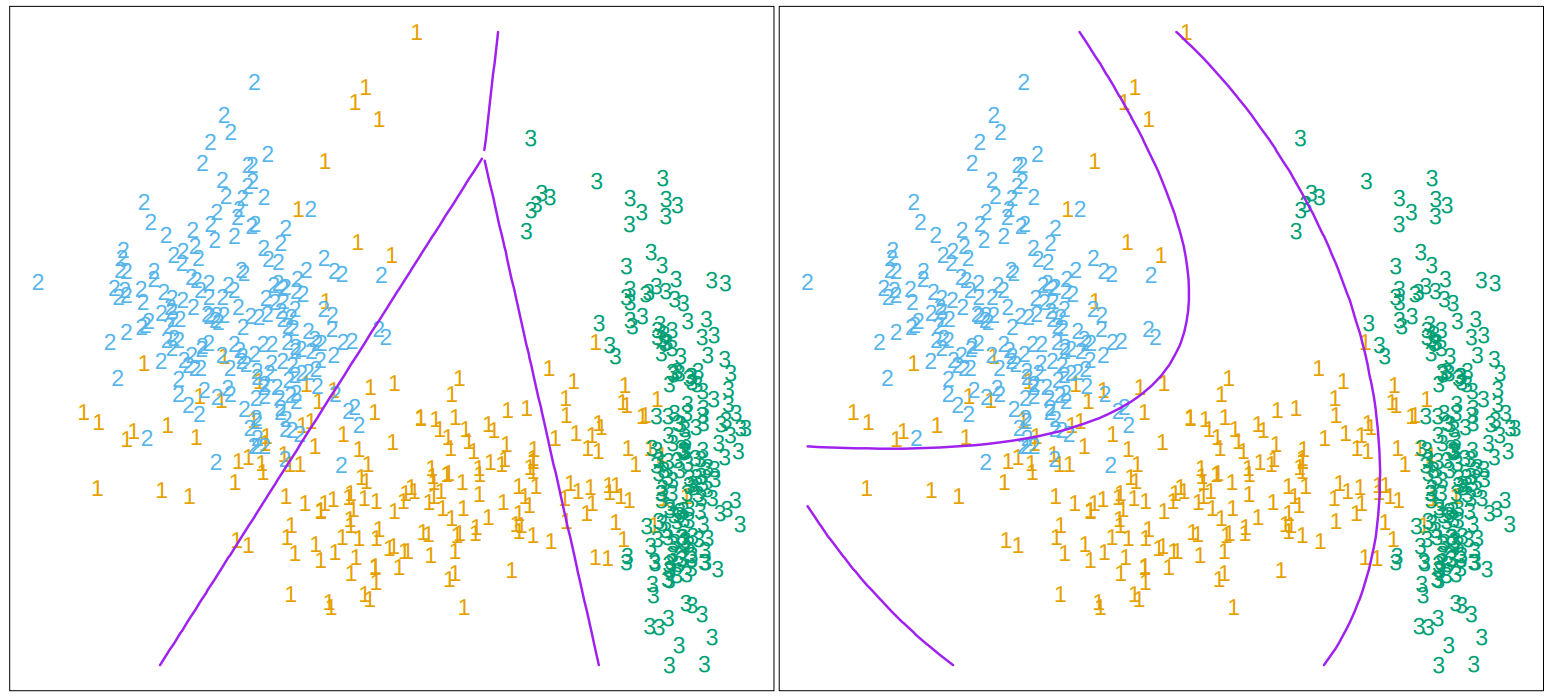
\includegraphics[width=\textwidth]{AugmentedFeatures.png}
\end{frame}


\begin{frame}{Linear Regression for Classification}
\begin{itemize}

\item[•] Indicator matrix $\mathbf{Y} \in \mathbb{R}^{NxK}$ with one-hot encoded class targets in rows

\vspace{0.2cm}
\item[•] Closed-form solution for weight matrix $\mathbf{B} \in \mathbb{R}^{(p+1)xK}$:
\begin{equation*}
\hat{\mathbf{B}} = (\mathbf{X}^T\mathbf{X})^{-1}\mathbf{X}^T\mathbf{Y}
\end{equation*}

\vspace{0.2cm}
\item[•] Classification via 
\begin{equation*}
\hat{f}(x)^T=(1,x^T)\hat{\mathbf{B}}
\end{equation*}
\begin{equation*}
\hat{G}(x) = argmax_{k \in \mathcal{G}} \hat{f}_k(x)
\end{equation*}

\end{itemize}
\end{frame}

\begin{frame}{Problems with Linear Regression Approach}
\begin{itemize}
\item[•] Limited interpretability of $\hat{f_k}(x)$ as $Pr(G=k|X=x)$, negative and greater 1 values possible
\item[•] Class masking effects

\vspace{0.8cm}


\begin{columns}
\begin{column}{0.5\textwidth}
\begin{center}
Linear regression
\end{center}
\end{column}
\begin{column}{0.5\textwidth}
\begin{center}
Linear Discriminant Analysis
\end{center}
\end{column}
\end{columns}
\end{itemize}
\begin{figure}
\begin{flushleft}
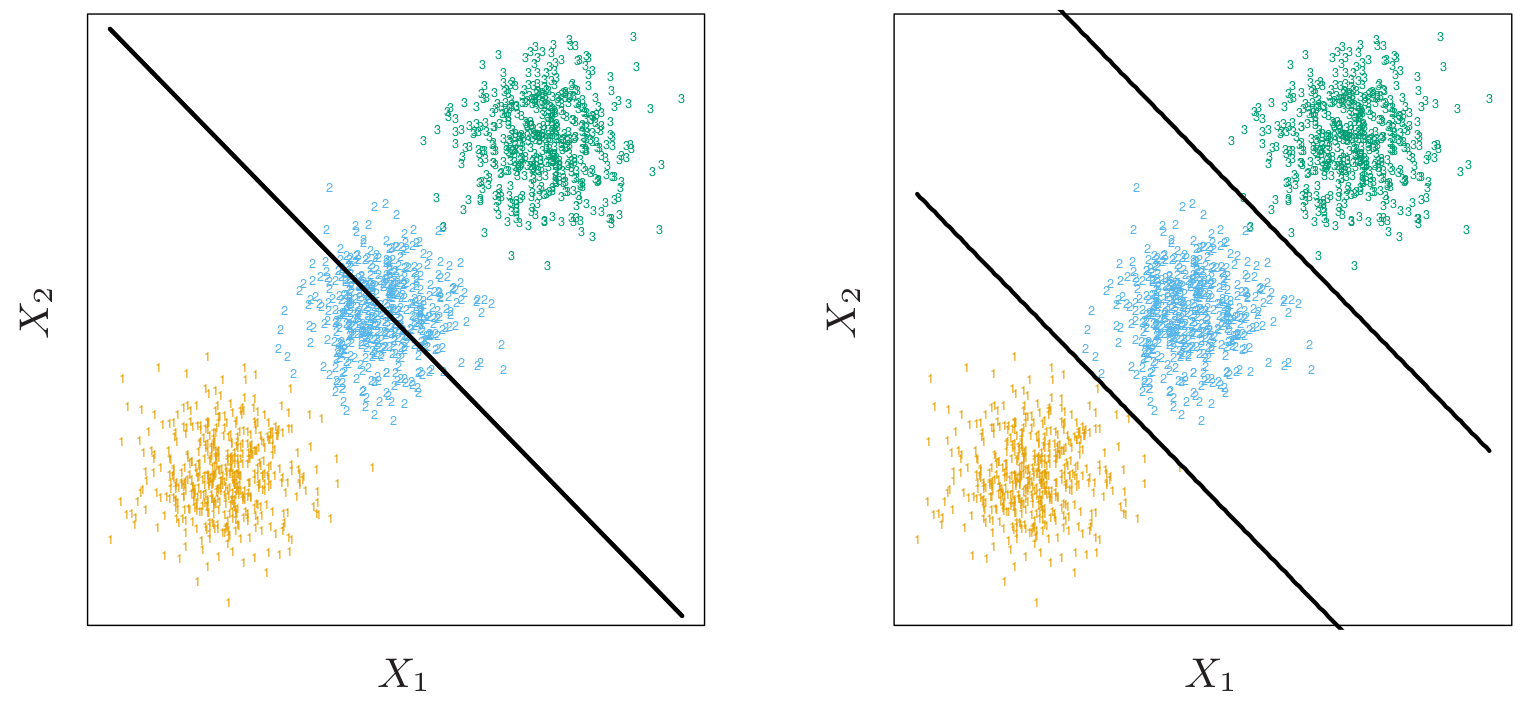
\includegraphics[width=0.9\textwidth]{Masking1.png}
\end{flushleft}
\end{figure}
\end{frame}

\begin{frame}{Effects of Masking}
\begin{figure}
\centering
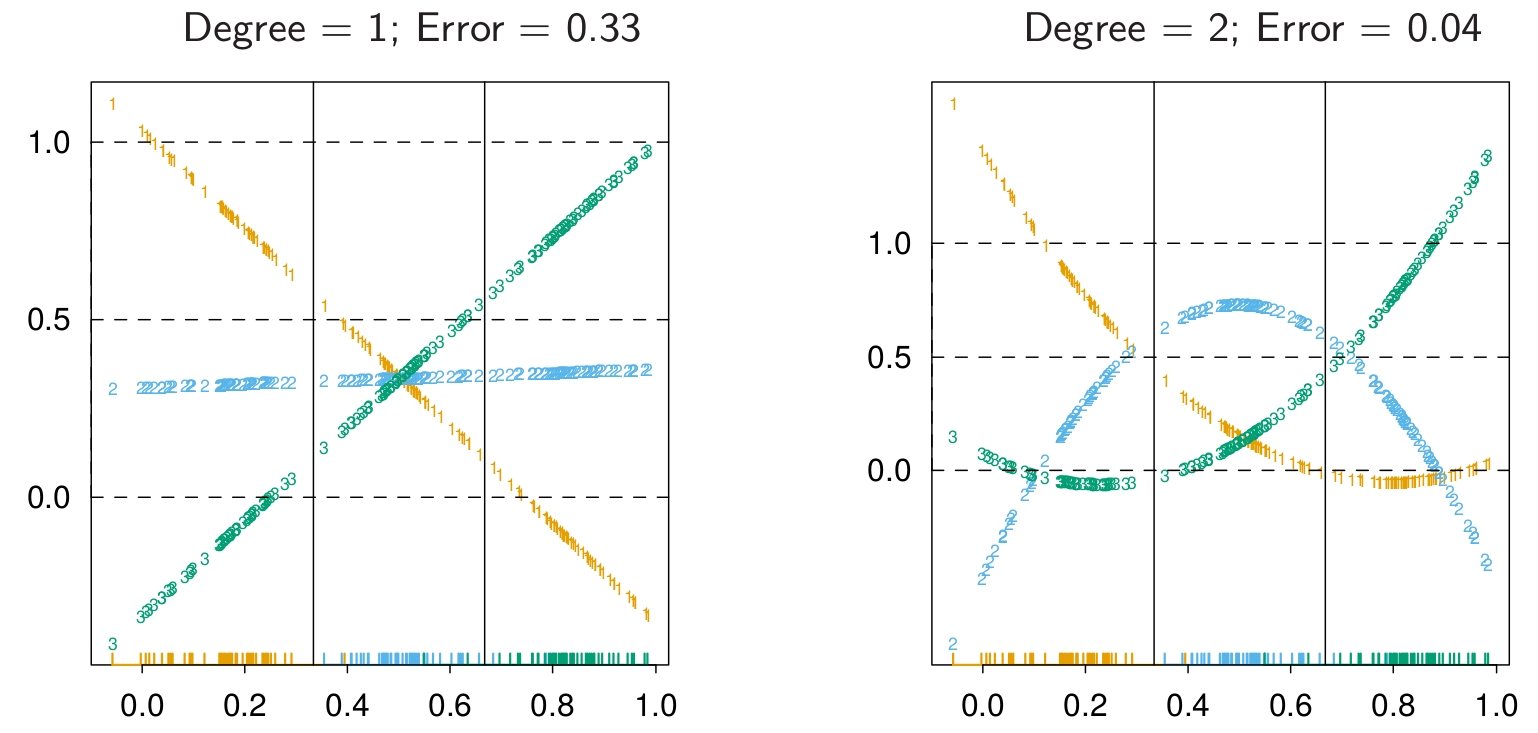
\includegraphics[width=\textwidth]{Masking2.png}
\end{figure}
\end{frame}

\begin{frame}{Linear Discriminant Analysis (LDA)}
\begin{itemize}
\item[•] Class posteriors $Pr(G|X)$ is needed for optimal classification
\item[•] With class-conditional density $f_k(x)=Pr(X=x|G=k)$ \\ and prior $\pi_k = Pr(G=k)$, 
\begin{equation*}
Pr(G=k|X=x)=\frac{f_k(x)\pi_k}{\sum_{j=1}^{K}f_j(x)\pi_j}
\end{equation*}
\item[•] LDA assumes mutliavriate Gaussians as class conditional densities with common covariance matrices $\Sigma_k = \Sigma \forall k \in K$
\end{itemize}
\end{frame}

\begin{frame}{Estimate Parameters of Gaussian Distribution}
\begin{equation*}
f_k(x)=\frac{1}{(2\pi)^{p/2}|\Sigma_k|^{1/2}}e^{-\frac{1}{2}(x-\mu_k)^T\Sigma_k^{-1}(x-\mu_k)}
\end{equation*}
with
\begin{equation*}
\hat{\pi_k} = \frac{N_k}{N}
\end{equation*}
\begin{equation*}
\hat{\mu_k}=\sum_{g_i=k}\frac{x_i}{N_k}
\end{equation*}
\begin{equation*}
\hat{\Sigma}=\sum_{k=1}^K\sum_{g_i=k}\frac{(x_i-\hat{\mu}_k)(x_i-\hat{\mu}_k)^T}{N-K}
\end{equation*}
\end{frame}

\begin{frame}{Linear Discriminant Functions}
\begin{itemize}
\item[•] To compare two classes j and k, it sufficies to compare log ratio:
\begin{equation*}
\log\frac{Pr(G=j|X=x)}{Pr(G=k|X=x)} 
\end{equation*}
\begin{equation*}
= \log\frac{\pi_j}{\pi_k}-\frac{1}{2}(\mu_j+\mu_k)^T\Sigma^{-1}(\mu_j-\mu_k) + x^T \Sigma^{-1}(\mu_k-\mu_l)
\end{equation*}
\item[•] Decision rule can be formulated as 
\begin{equation*}
G(x) = argmax_k\delta_k(x)
\end{equation*}
with
\begin{equation*}
\delta_k(x) = \log\pi_k-\frac{1}{2}\mu_k^T\Sigma^{-1}\mu_k+x^T\Sigma^{-1}\mu_k
\end{equation*}
\end{itemize}
\end{frame}

\begin{frame}{LDA Result}
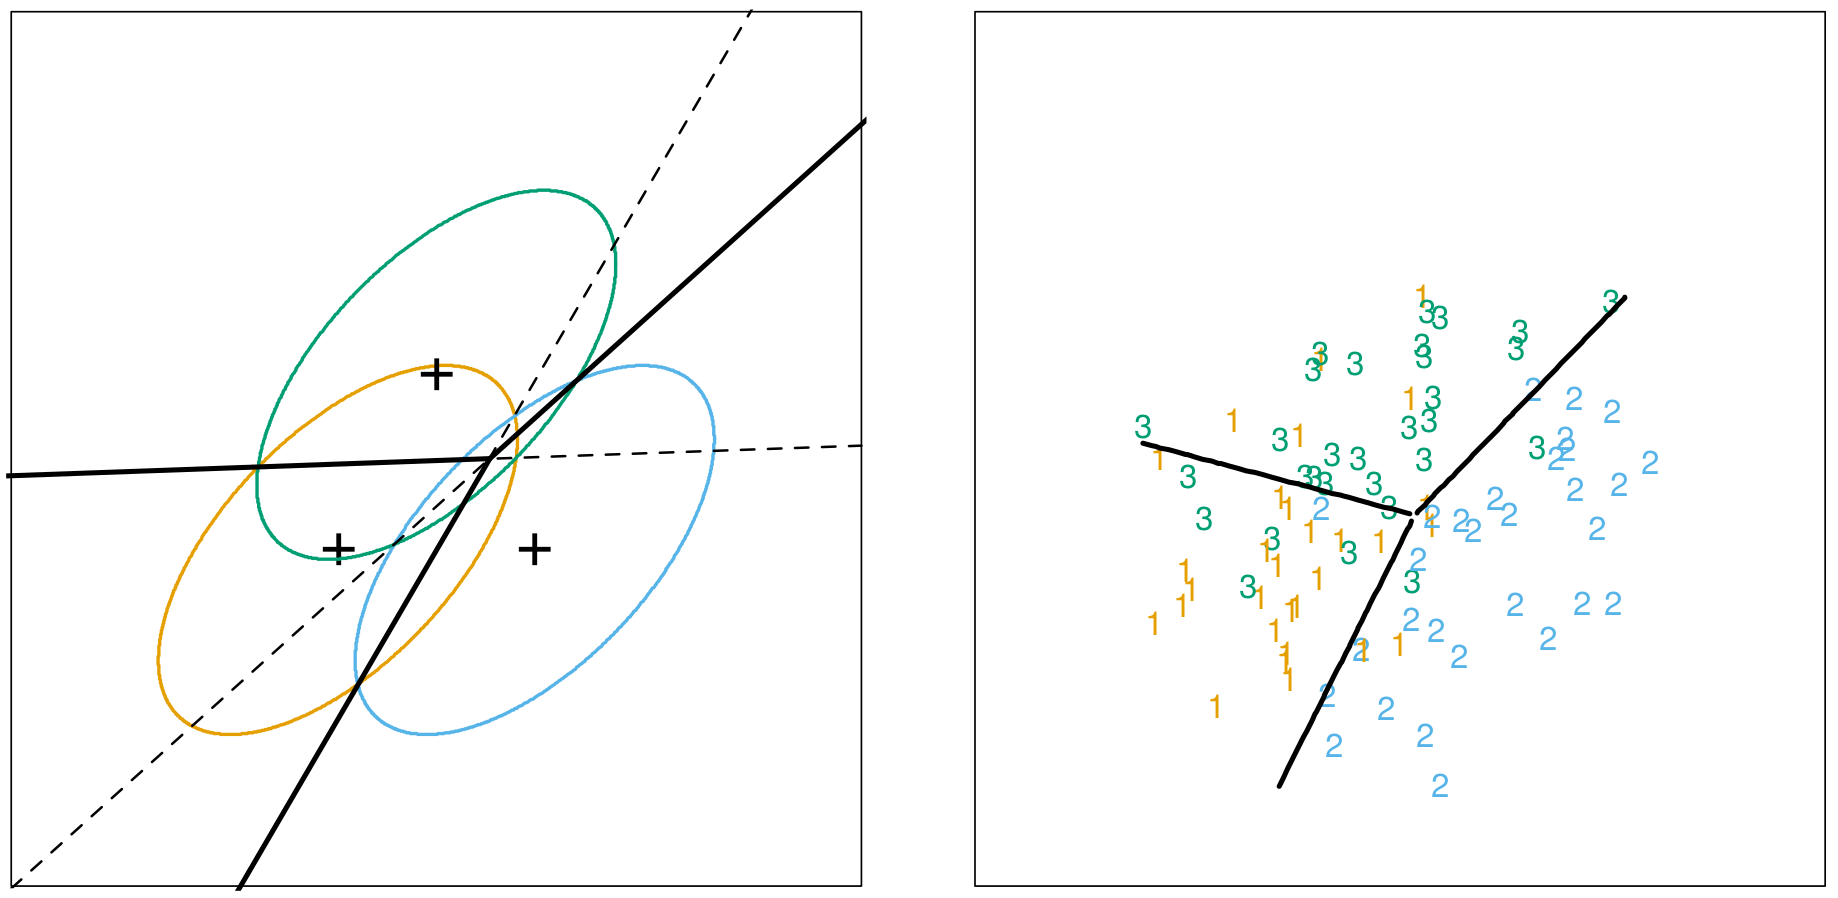
\includegraphics[width=\textwidth]{LDA_result.png}
\begin{columns}
\begin{column}{0.5\textwidth}
\begin{center}
Bayes decision boundaries
\end{center}
\end{column}
\begin{column}{0.5\textwidth}
\begin{center}
LDA decision boundaries on 20 samples
\end{center}
\end{column}
\end{columns}
\end{frame}

\begin{frame}{LDA vs QDA}
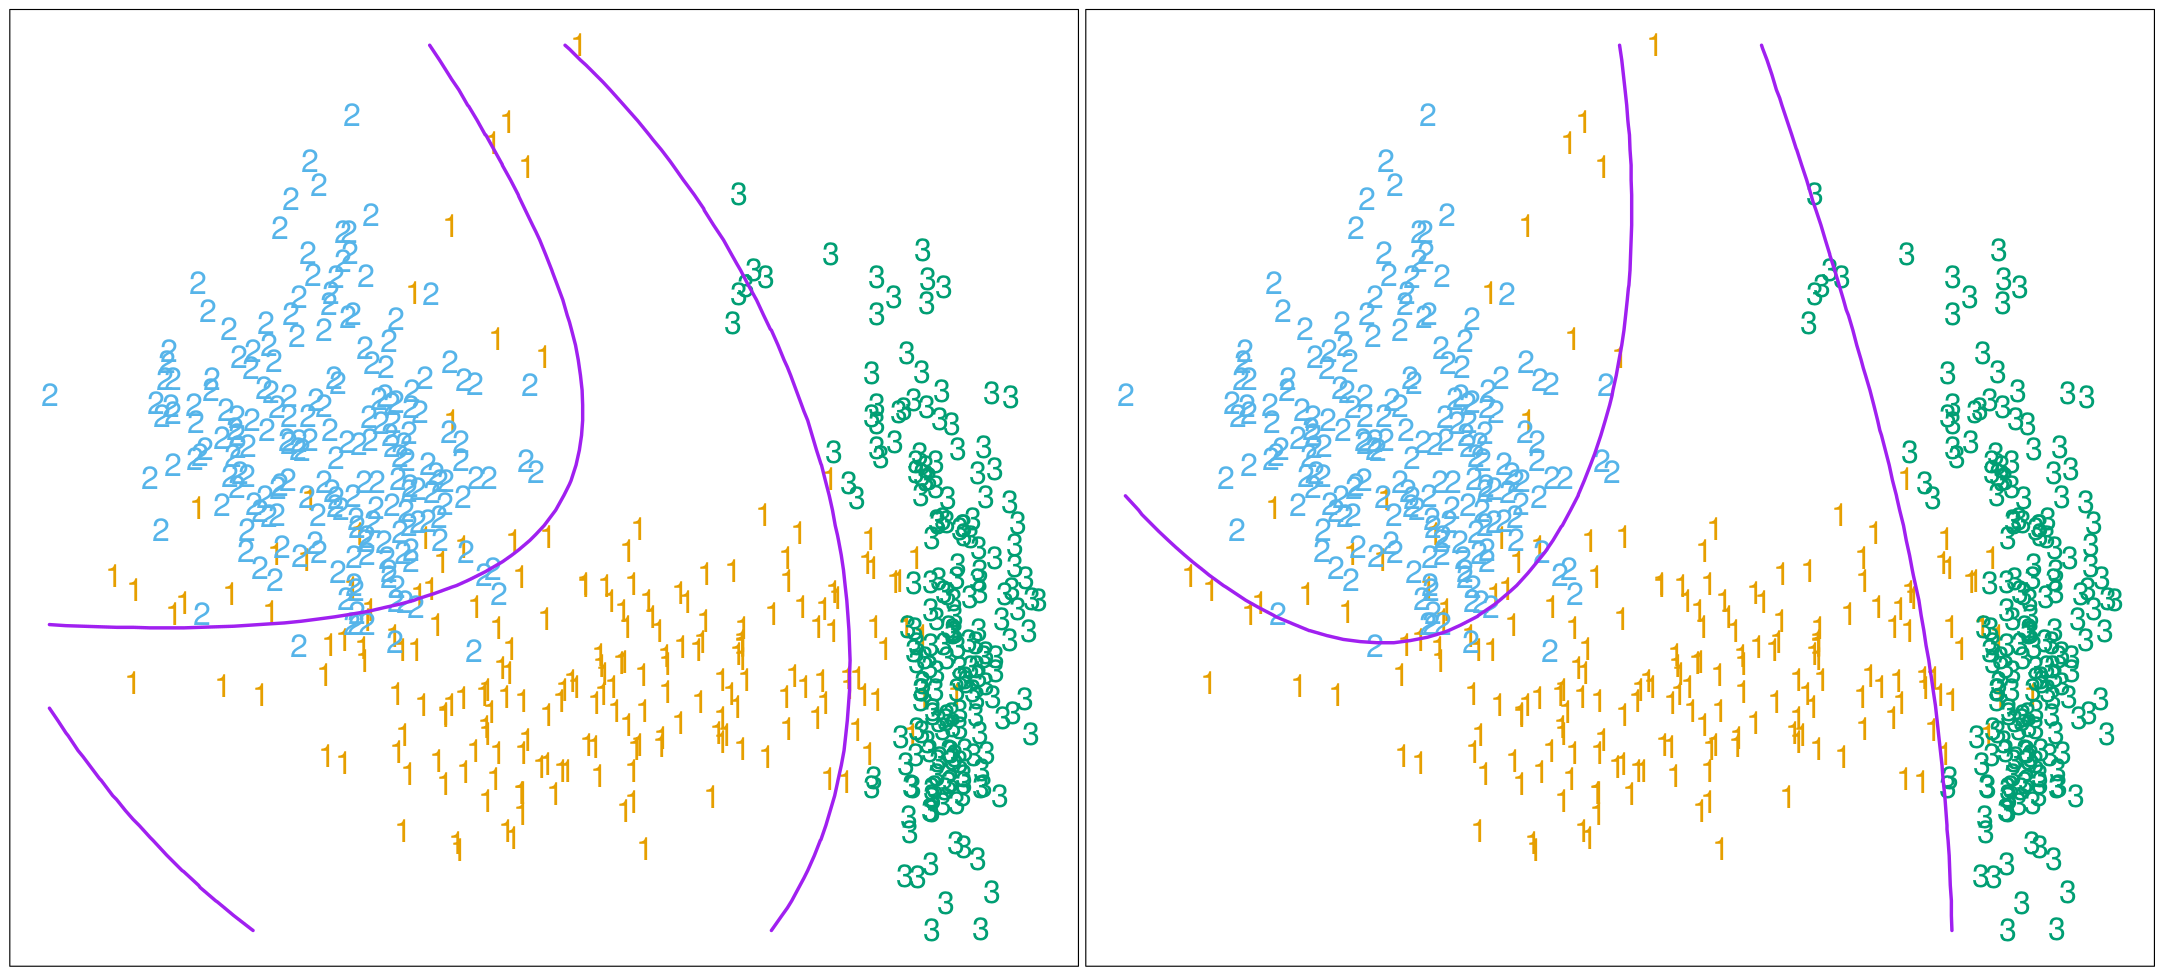
\includegraphics[width=\textwidth]{LDAQDA.png}
\begin{columns}
\begin{column}{0.5\textwidth}
\begin{center}
LDA\\ with augmented feature space
\end{center}
\end{column}
\begin{column}{0.5\textwidth}
\begin{center}
QDA $(\Sigma_j \neq \Sigma_k)$
\end{center}
\end{column}
\end{columns}
\end{frame}

\begin{frame}{Logistic Regression}
Squash network output $\mathbb{R}\rightarrow [0,1]$ using
\begin{equation*}
\sigma(x) = \frac{1}{1+e^{-x}}
\end{equation*}
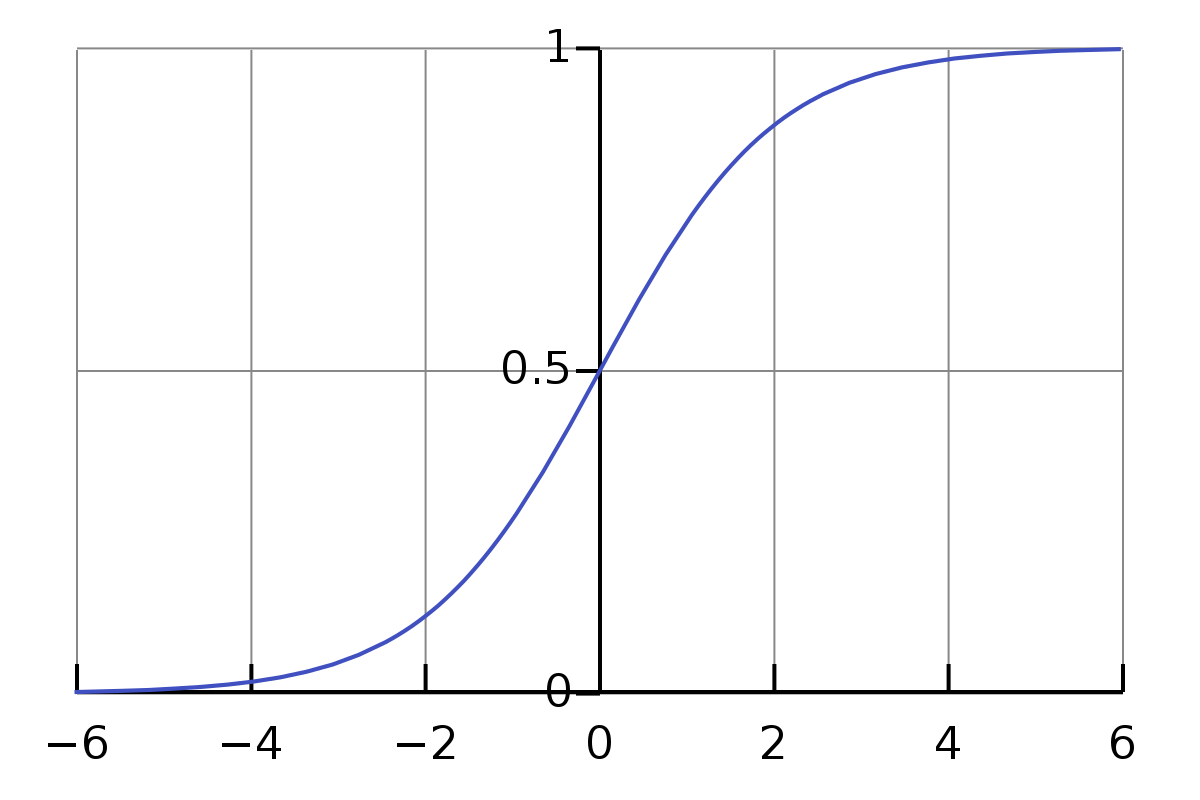
\includegraphics[width=\textwidth]{logistic_function.png}

\end{frame}

\begin{frame}{Fitting Logistic Regression}

\end{frame}

\begin{frame}{Example: South African Hearth Disease}

\begin{columns}
\begin{column}{0.5\textwidth}
\begin{center}
Model selection strategies:
\begin{itemize}
\item[1)] Remove independent variable with least significant coefficient
\item[2)] Refit model with each variable removed, perform analysis of deviance
\end{itemize}
\end{center}
\end{column}
\begin{column}{0.5\textwidth}
\begin{center}
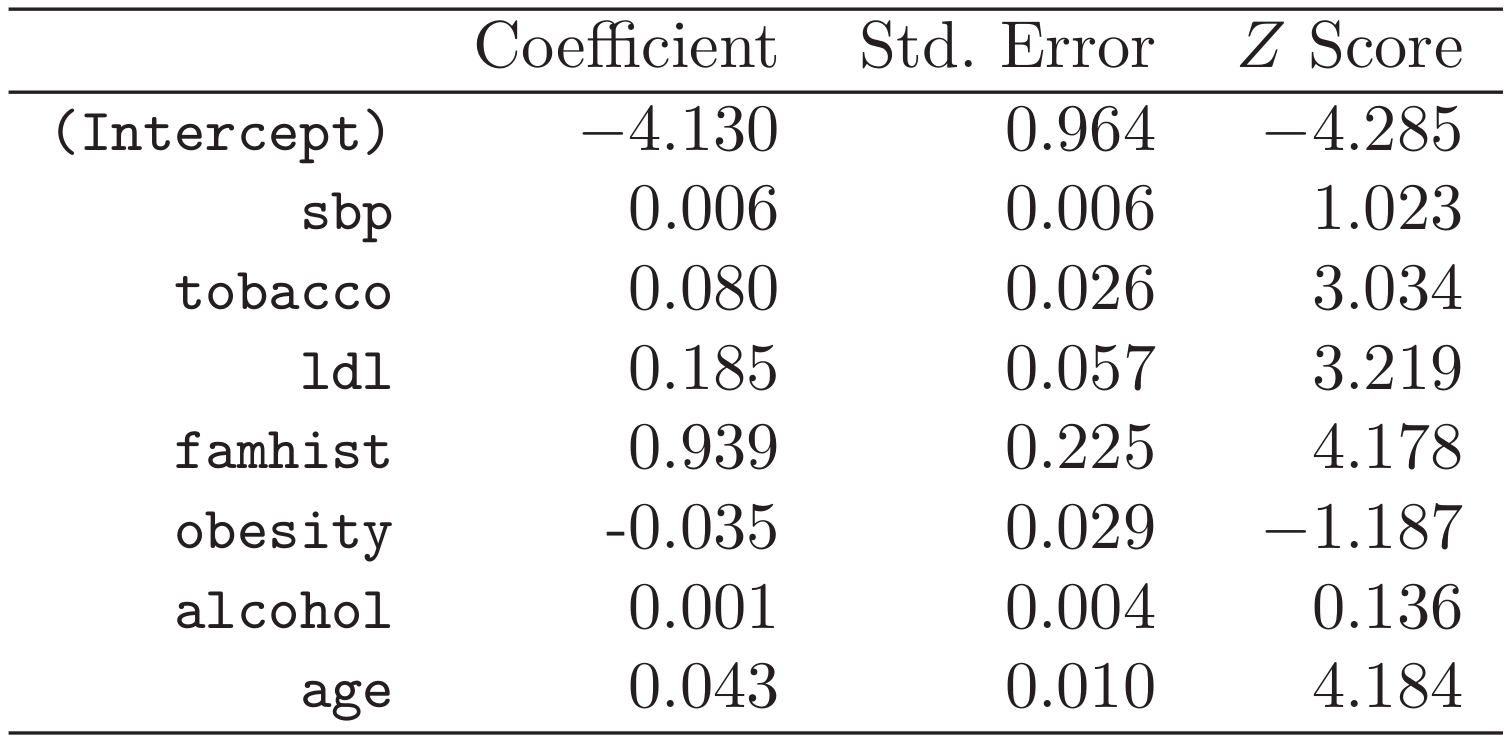
\includegraphics[width=\textwidth]{heart_results_all.png}
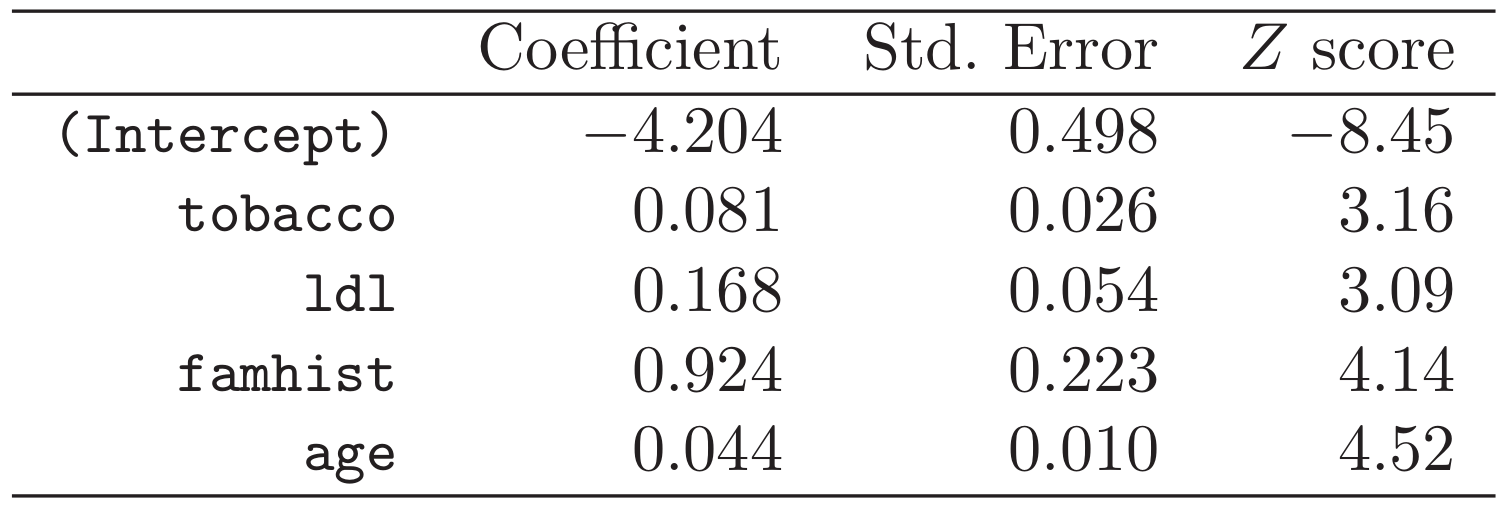
\includegraphics[width=\textwidth]{hearth_results_selected.png}
\end{center}
\end{column}
\end{columns}
\end{frame}

\begin{frame}{Example: South African Hearth Disease}
\begin{center}
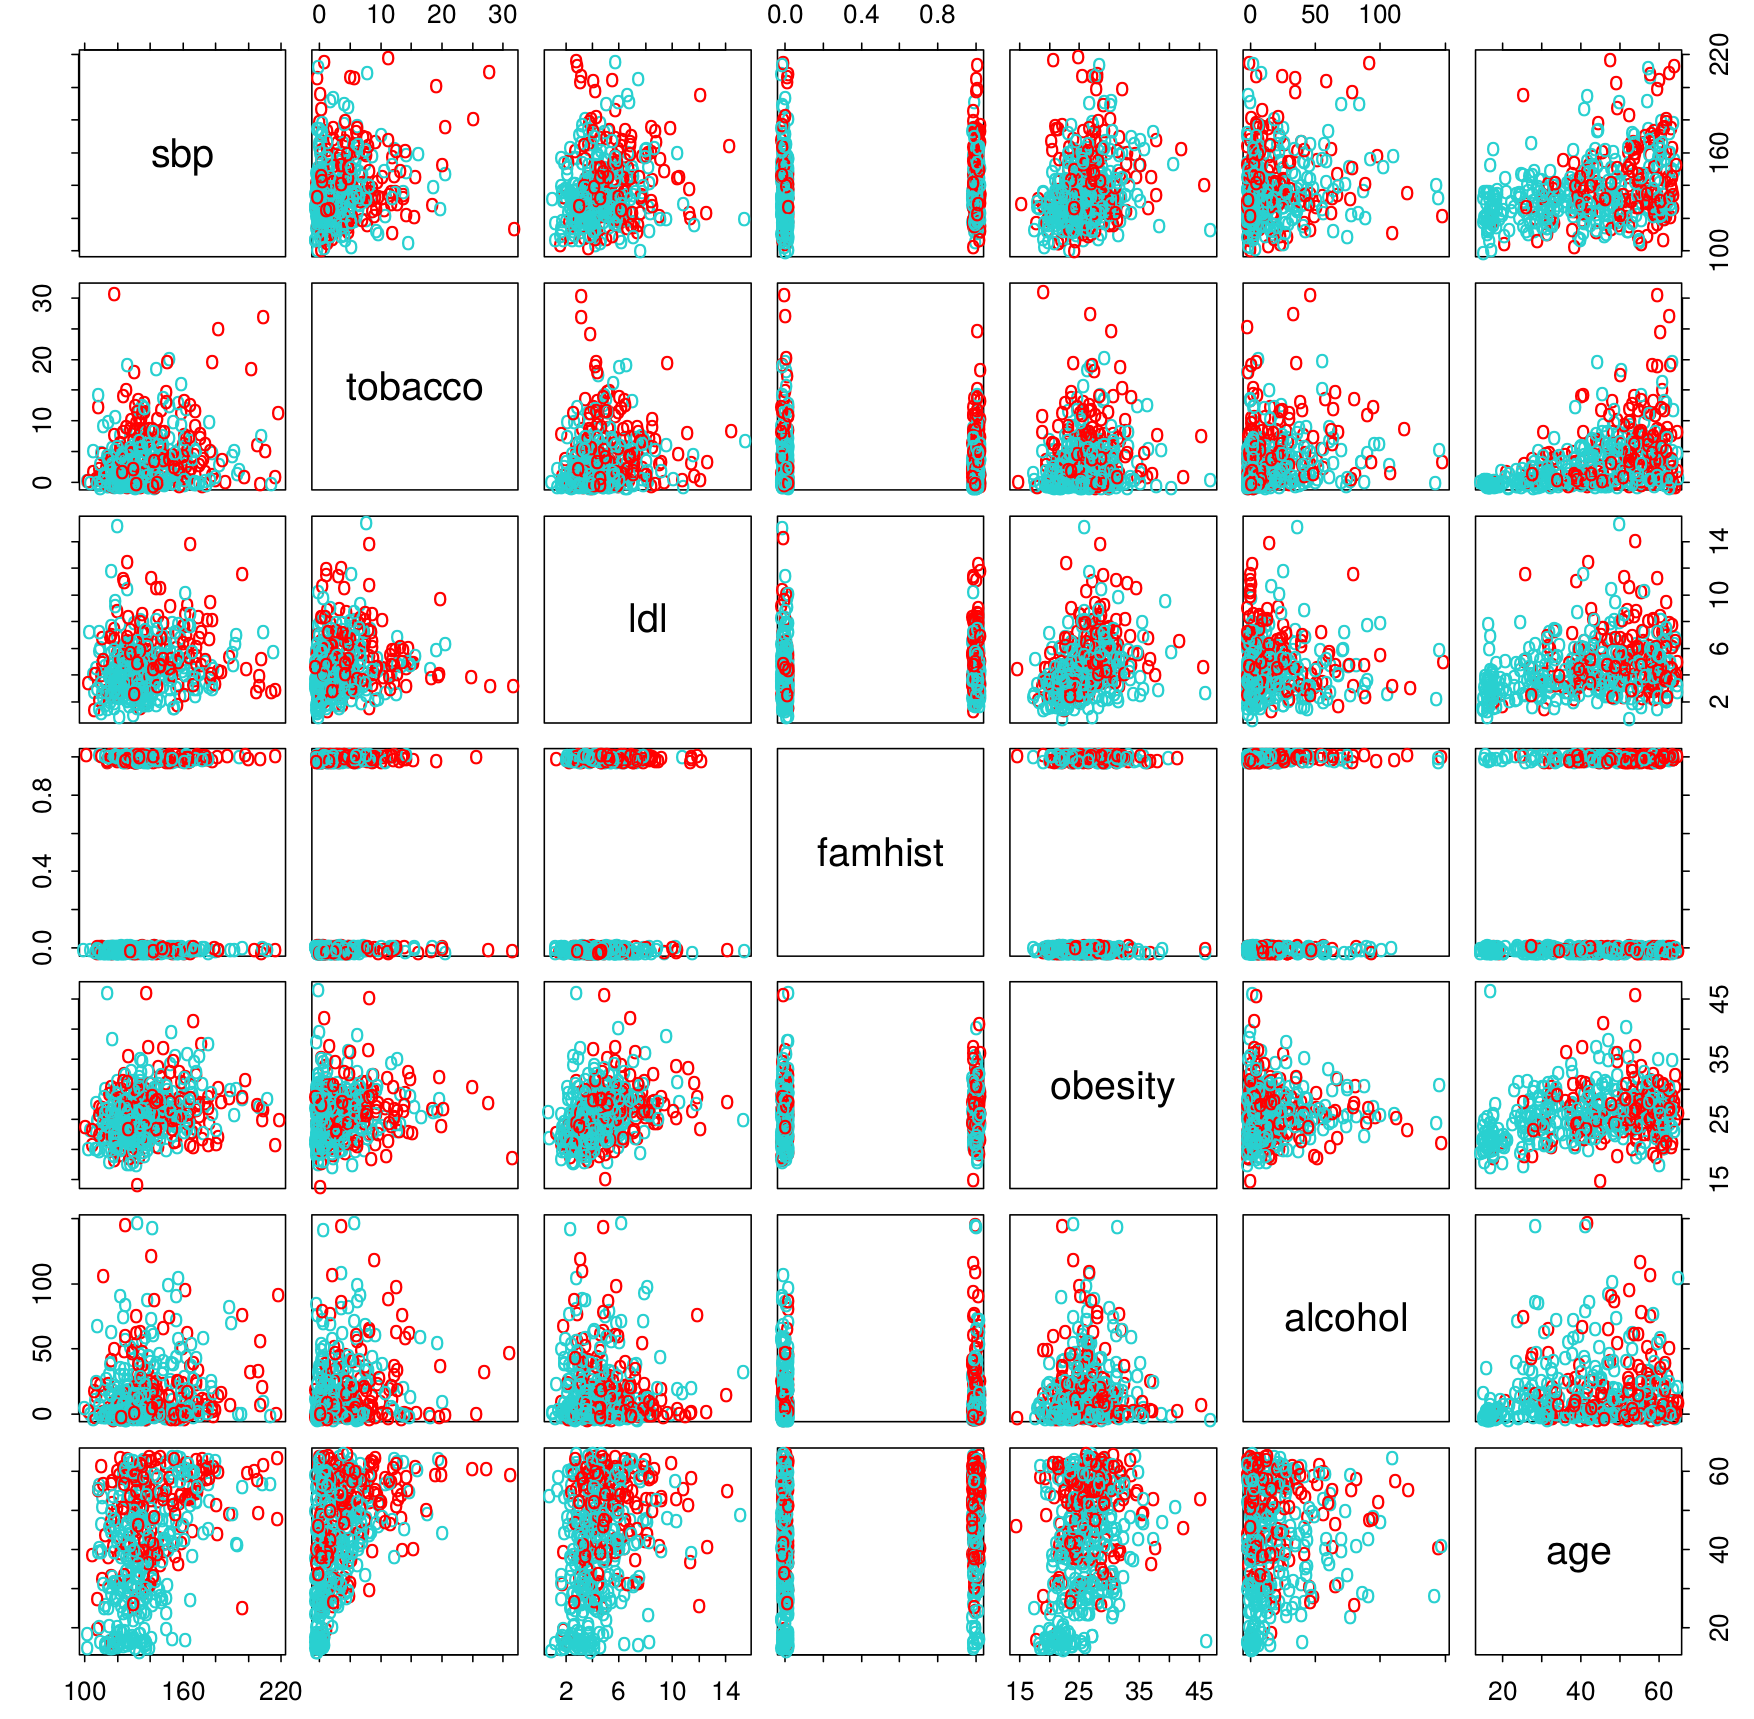
\includegraphics[width=0.6\textwidth]{scatter.png}
\end{center}
\end{frame}


\begin{frame}{$L_1$ Regularized Logistic Regression}
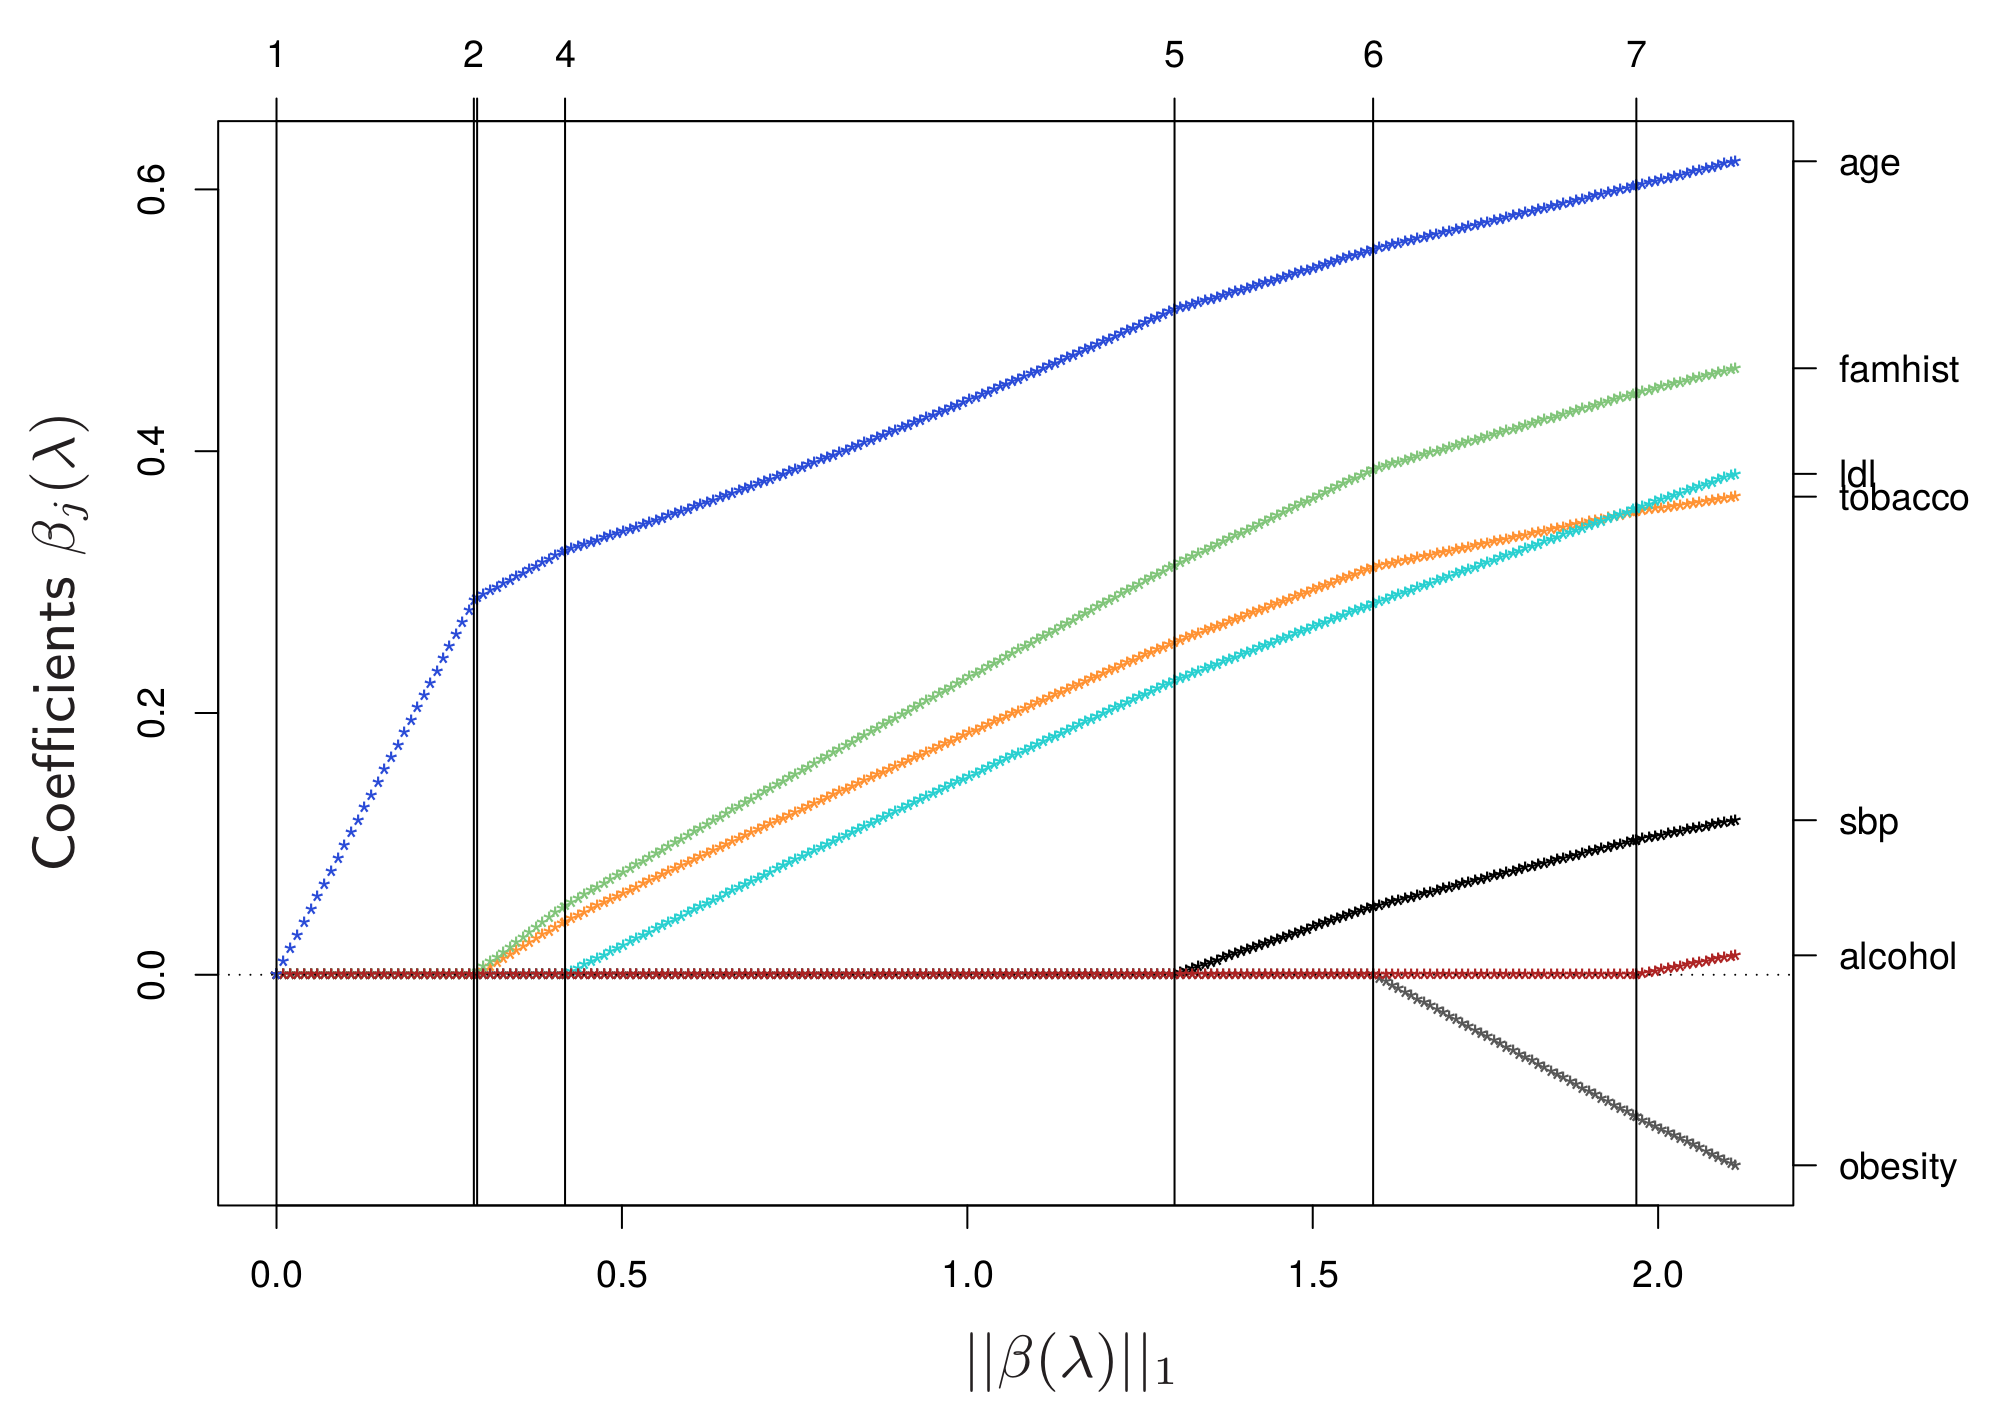
\includegraphics[width=\textwidth]{L1.png}
\end{frame}

\begin{frame}{Logistic Regression vs. LDA}

\end{frame}



\end{document}
